\section{Motivation: The State Dispersal Problem}
\label{sec:motivation}

\subsection{A Pattern, Not an Anecdote}

The two cases described above---the network monitor and the time-tracking
application---exhibit the same structural pathology by different means. We call
it \emph{state dispersal}: the condition in which the behavioral state of a
system is encoded implicitly, in fragments, across locations that have no
formal relationship to one another.

State dispersal is not a new problem. It is the problem that object-oriented
programming was supposed to solve, and solved only partially: encapsulation
prevents external mutation but does not prevent internal duplication. A boolean
flag checked in four places is dispersed state even if every check is inside
the same module. The language permits it. The programmer produces it. The LLM
faithfully reproduces it, because the corpus from which it learned was written
by the same programmers.

\subsection{Case~1 --- MonitoreoRed}
\label{sec:monitoreo}

MonitoreoRed is a home network monitoring system built over Prometheus, Grafana,
Blackbox Exporter, Node Exporter, and Docker, running on a fourteen-device home
network. It was built collaboratively with Claude in a single session, from an
empty directory, with no prior scaffolding.

The functional result was genuine: the system monitored device availability,
collected metrics, and exposed a Grafana dashboard. An unrequested feature---
vendor identification from MAC address using the IEEE OUI registry---was
introduced by Claude during the session and retained as a contribution.

The structural problem was discovered later. Device state was represented in
three incompatible forms:

\begin{table}[h]
  \caption{Three representations of device state in MonitoreoRed, none of which
           captures the full state machine.}
  \label{tab:monitoreo-state}
  \small
  \begin{tabular}{p{1.9cm}p{2.2cm}p{3.5cm}}
    \toprule
    Representation & Location & What it captures \\
    \midrule
    JSON snapshot  & \texttt{devices.json} & Known devices at last scan \\
    Time-series    & Prometheus TSDB            & Metrics (latency, reachability) --- not states \\
    Point-in-time  & \texttt{ping\_check.py}, \texttt{network\_scan.py} & Instantaneous presence --- discarded after check \\
    \bottomrule
  \end{tabular}
\end{table}

\begin{sloppypar}
There was no model of the transition \texttt{KnownDevice} $\to$ \texttt{Absent}
$\to$ \texttt{ActiveAlert}. The transition from ``this device was present'' to
``this device has been absent long enough to warrant an alert'' was not
representable in any of the three layers. It had to be reconstructed each time
from the intersection of three independently maintained data structures---a
reconstruction that neither the system nor any assisting LLM could perform
mechanically, because the rule was nowhere written down.
\end{sloppypar}

\begin{figure}[h]
  \centering
  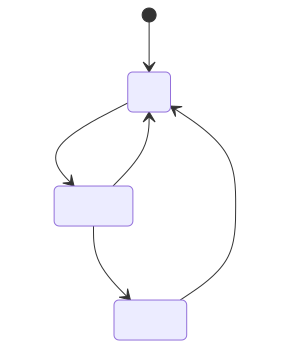
\includegraphics[width=0.825\linewidth]{figures/monitoreored}
  \caption{MonitoreoRed state model: three states and the storage layers
           present (\textbf{+}) or absent (\textbf{--}) for each.}
  \label{fig:monitoreored}
\end{figure}


The \texttt{claude-flow} framework, which uses a fifteen-agent coordination
model to manage complex AI workflows~\cite{claudeflow2024}, represents one
response to this kind of problem: if the system is too complex for a single
model to reason about, distribute the reasoning. We think this approach does
not address state dispersal. The problem is not cognitive capacity---it is the
absence of a shared, formal account of what the system's state is. Adding
agents without adding a state model produces a system that is more complex
without being more coherent.

\subsection{Case~2 --- CronometroPSP}
\label{sec:cronometro}

CronometroPSP is a personal software process (PSP) time-tracking application
with a mobile-first HTML/JavaScript interface. It was also built with Claude.
Its behavioral complexity is dominated by a modal UI with two distinct
interaction modes: normal operation (\texttt{NormalMode}) and activity editing
(\texttt{EditMode}).

The flag \texttt{editMode} was checked in four independent locations:

\begin{enumerate}
  \item The card-tap handler in the main view.
  \item The activity-tab tap handler.
  \item The frequent-activities tab handler.
  \item A secondary card interaction path.
\end{enumerate}

In practice, location~4 was missing the guard. On mobile, tapping a card in
edit mode opened the session dialog instead of the edit dialog. The bug was
real, reproducible, and intermittent (it required a specific navigation path
to trigger).

When Claude was asked to diagnose and fix the bug, the process was
disproportionate to the defect. The reason was not computational but
architectural: Claude had no privileged access to the code it had written. The
code was as opaque to it as any other code of similar length and complexity.
Reconstructing the intent of four conditional branches scattered across several
hundred lines required the same heuristic reasoning that would have been
required for foreign code---with the same probability of misdiagnosis.

\begin{figure}[h]
  \centering
  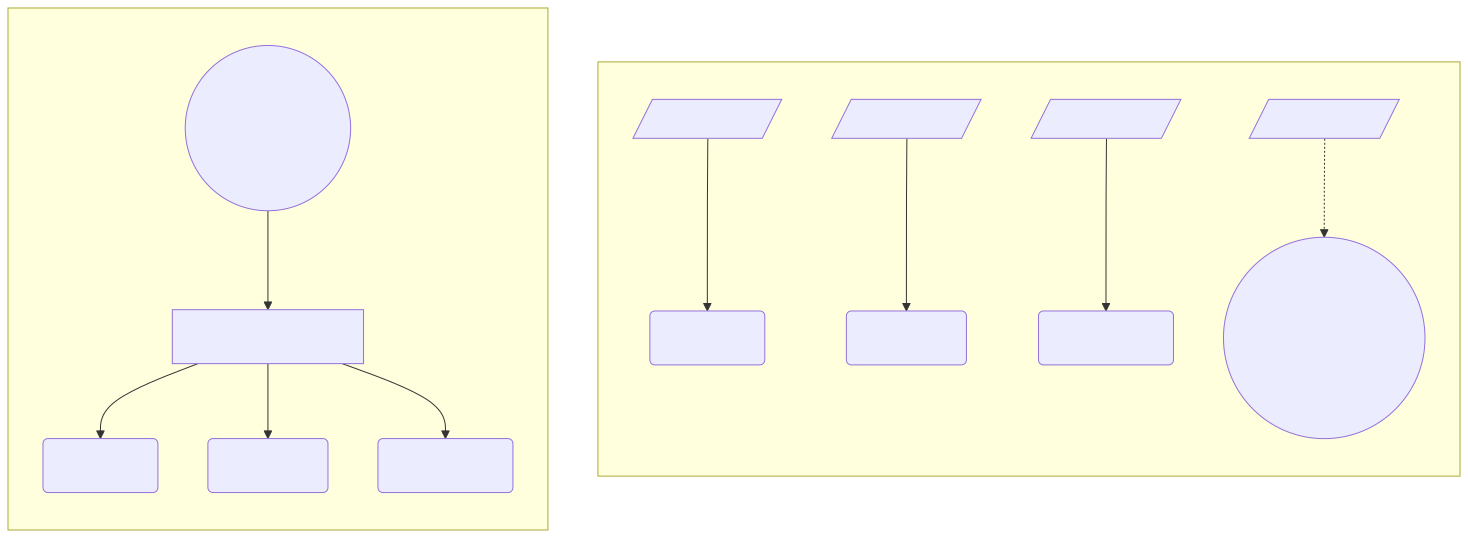
\includegraphics[width=\linewidth]{figures/dispersed}
  \caption{Comparison of the dispersed boolean flag pattern versus the Trenza polymorphic alternative.}
  \label{fig:dispersed}
\end{figure}

The correct fix was structural: \texttt{editMode} should not have been a
boolean flag. It should have been the identity of a polymorphic object. The
four conditional branches should have been four method implementations, selected
at construction time by a factory. In that design, the missing case at
location~4 would have been a missing method implementation---a compilation
error, not a runtime defect.

\subsection{The Common Structure}
\label{sec:pattern}

Both cases exhibit the same pattern:

\begin{quote}
\itshape
A behavioral condition that should be a named, first-class entity in the
system's design is instead encoded as a recurrence---a flag checked in multiple
places, a state reconstructed from multiple sources---with no formal guarantee
of consistency across occurrences.
\end{quote}

This pattern is not detectable by conventional static analysis, because no
individual occurrence is incorrect. It is detectable only by reasoning about
the design, which requires knowing the design. In a human-LLM collaboration
where the LLM has no persistent memory of the design decisions it participated
in, that knowledge is unavailable without an external artifact that makes it
explicit.

Trenza is that artifact.

\medskip

\noindent\textbf{Generality.}
We observe that state dispersal is endemic to the LLM-assisted development
workflow for a structural reason: LLMs are trained on corpora written by humans
who routinely produce dispersed state, and have no mechanism---absent an
explicit schema---to detect when they are doing so. The corpus normalizes the
pattern. Without a DSL that forbids it, the pattern will recur regardless of
the capability of the model. This is not a limitation of current LLMs; it is a
consequence of the relationship between any statistical learner and the
distribution it was trained on. Formal constraint is the only leverage point.
